\section{Environment Definition}
One of the main reasons for the use of OpenAI Gym in this project is the ability to standardize the environments.
In this section each Gym environment will be described.

\subsection{Cartpole}
The cartpole environment is a very simple exercise, consisting of a pole in a cart moving on an horizontal plane, 
the objective is to balance this pole by applying a force on the right or left side of the cart making it move in the oposite direction.
\cite{cartpole}

\begin{figure}[H]
    \centering
    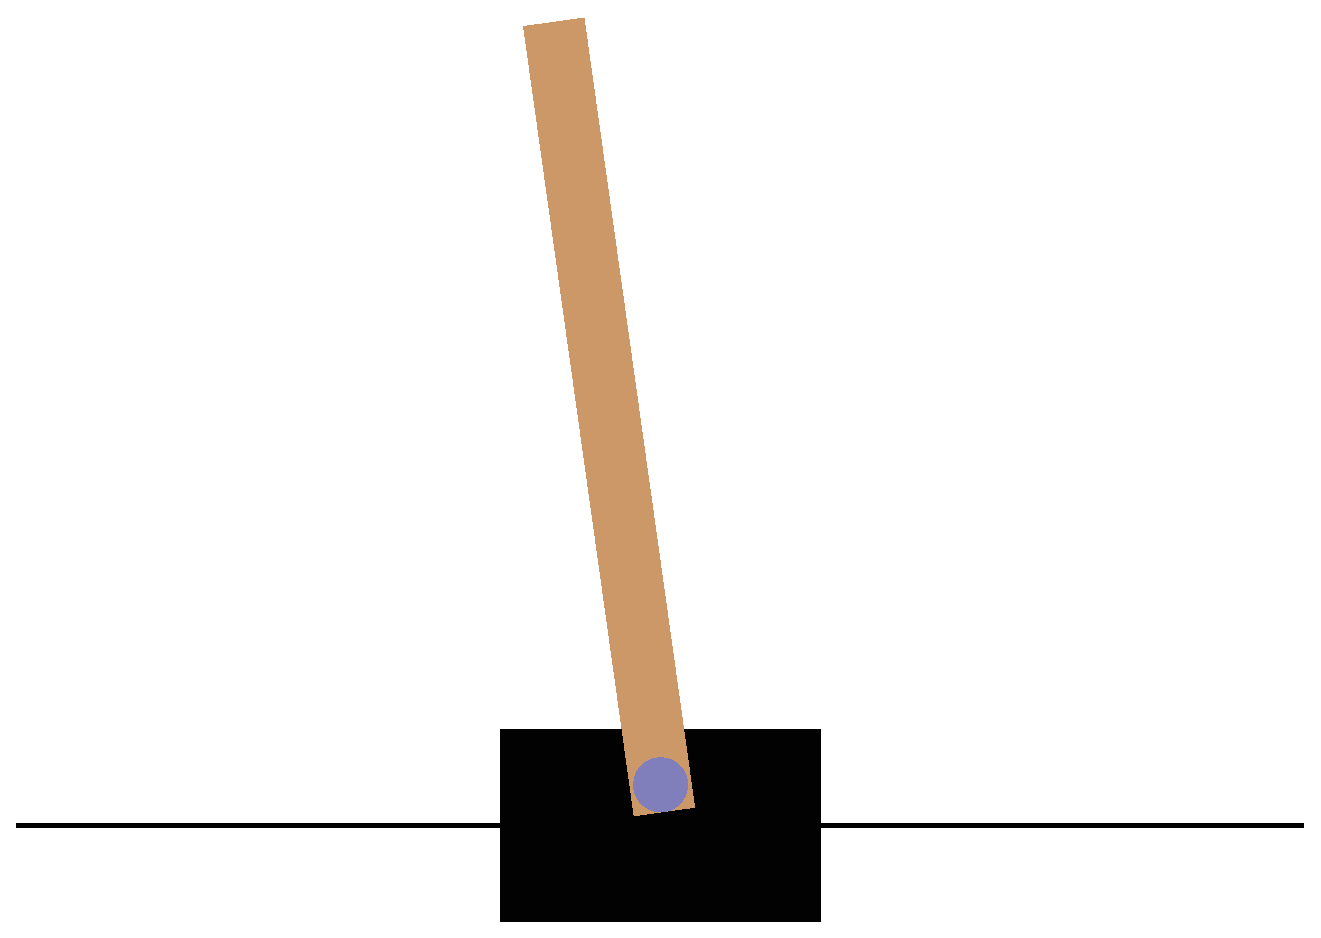
\includegraphics[scale=0.24]{cartpole}
    \caption{Rendered Cartpole Environment - OpenAI Gym}
\end{figure}

Cartpole Environment definition:
\begin{itemize}
    \item \textbf{Observation Space}
            \begin{table}[H]
                \caption{Observation Space for the Cartpole environment}
                \centering
                \begin{tabular}{|l|l|l|l|}
                \hline
                Num & Observation           & Min  & Max  \\ \hline
                0   & Cart Position         & -4.8 & +4.8 \\ \hline
                1   & Cart Velocity         & -Inf & +Inf \\ \hline
                2   & Pole Angle            & -24° & +24° \\ \hline
                3   & Pole Angular Velocity & -Inf & +Inf \\ \hline
                \end{tabular}
                \end{table}
    \item \textbf{Action Space} 
    \begin{table}[H]
        \caption{Action Space for the Cartpole environment}
        \centering
        \begin{tabular}{|l|l|}
        \hline
        Num & Action                 \\ \hline
        0   & Push cart to the left  \\ \hline
        1   & Push cart to the right \\ \hline
        \end{tabular}
        \end{table}
    \item \textbf{Reward:} In the cartpole environment the reward is attributed per timestep survived, being awarded 1 point per timestep.
    \end{itemize} 

\subsection{2D Walker}
The 2D environment requires a 2D Humanoid, this has been defined with 8 different joints, 2 in the shoulder, 2 in the hips, 2 in the knees and 2 for the ankles.
\begin{figure}[H]
    \centering
    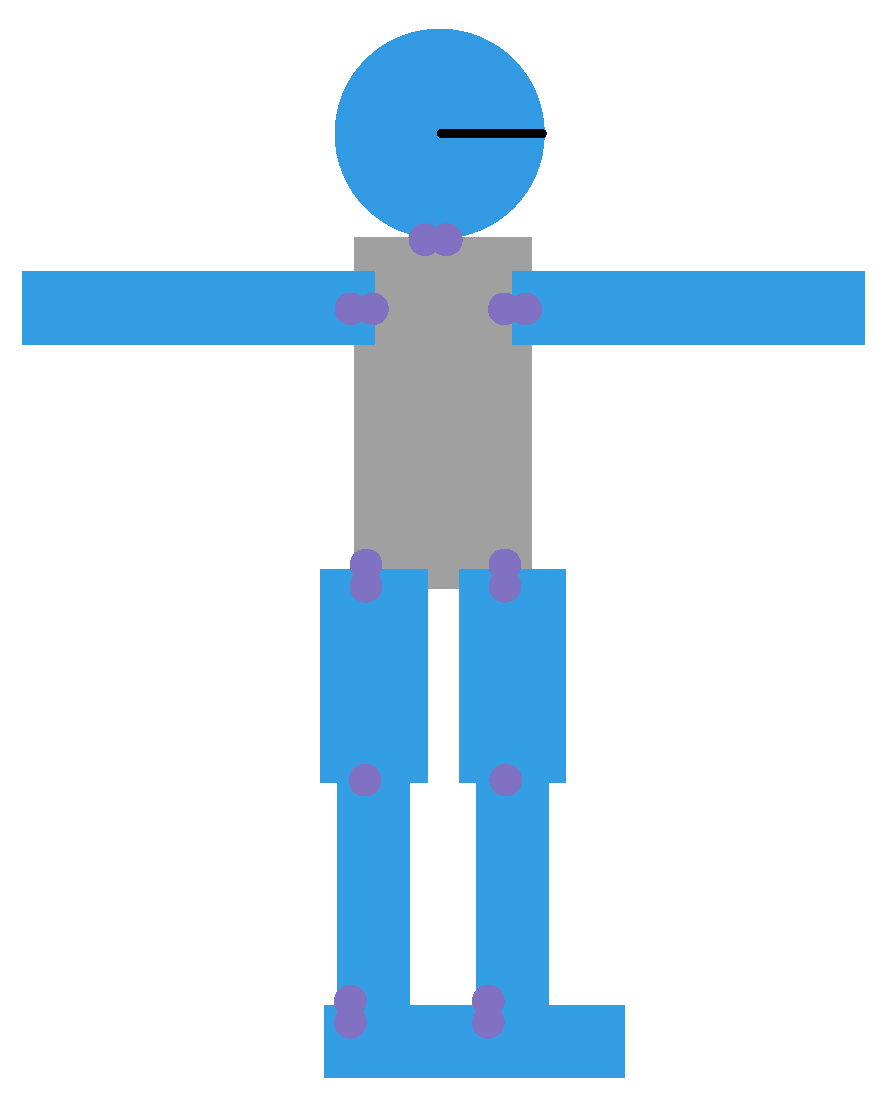
\includegraphics[scale=0.25]{humanoid-2d}
    \caption{Representation of 2D humanoid}
\end{figure}

Environment definition:
\begin{itemize}
    \item \textbf{Observation Space:} The Observation Space is a vector of size 8, containing the angles for each of the 8 joints of the humanoid.
    \begin{table}[H]
        \caption{Observation Space for the 2D Walker environment}
        \centering
        \begin{tabular}{|l|l|l|}
        \hline
        Observation           & Min  & Max  \\ \hline
        Joint Position         & -20° & +20° \\ \hline

        \end{tabular}
        \end{table}

    \item \textbf{Action Space:} 
    \begin{table}[H]
        \caption{Action Space for the 2D Walker environment}
        \centering
        \begin{tabular}{|l|l|}
        \hline
        Num & Action                 \\ \hline
        0   & Move the joint counterclockwise  \\ \hline
        1   & Maintain joint position \\ \hline
        2   & Move the joint clockwise \\ \hline
        \end{tabular}
        \end{table}
    \item \textbf{Reward:} 
    \begin{table}[H]
        \caption{Reward system for the 2D Walker environment}
        \centering
        \begin{tabular}{|l|l|}
        \hline
        Action & Points                 \\ \hline
        Moves Back   &  - 2  \\ \hline
        Stays in Place   & -1 \\ \hline
        Moves Forward   & 1 \\ \hline
        Loses contact with the ground & cumulative -2 \\ \hline
        Reaches target & 10 \\ \hline
        Falls & -10 \\ \hline
        \end{tabular}
        \end{table}
    
\end{itemize}

\subsection{3D Walker}
In the 3D environment, the robot needs to simulate the one used by the Bold Hearts team, given that the team already uses a simulator, gazebo, this will be used to interact with the robot given that it provides ROS2 integration.
\begin{figure}[H]
    \centering
    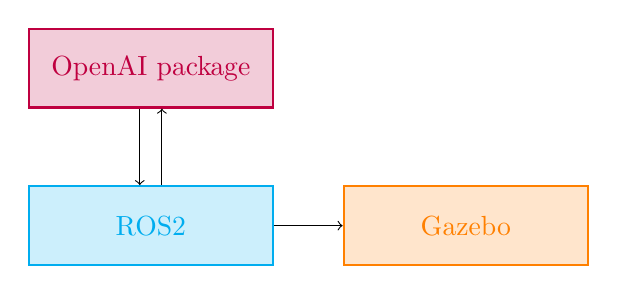
\begin{tikzpicture}[every node/.style=draw]
        \node[rectangle, 
        draw, 
        thick,
        minimum width = 3.1cm,
        minimum height = 1cm,
        color=cyan,
        fill=cyan!20] (A) at (0,0) {ROS2};
        \node[rectangle, 
        draw, 
        thick,
        minimum width = 3.1cm,
        minimum height = 1cm,
        color=purple,
        fill=purple!20] (B) at (0,2) {OpenAI package};
        \node[rectangle, 
        draw, 
        thick,
        minimum width = 3.1cm,
        minimum height = 1cm,
        color=orange,
        fill=orange!20] (C) at (4,0) {Gazebo};

        \draw [->] ([xshift=-4]B.south) to  node [midway,left, draw=none]{} ([xshift=-4]A.north);
        \draw [<-] ([xshift=4]B.south) to  node [midway,left, draw=none]{} ([xshift=4]A.north);
        \draw [->] (A.east) to  node [midway,left, draw=none]{} (C.west);
    
    \end{tikzpicture}
    \caption{Integration of ROS2, Gazebo and OpenAI Gym}
\end{figure}

To achieve this integration, OpenAI Gym should be able to subscribe ROS2 topics containing the world observations. 
The OpenAI Gym should also be able to publish to ROS2 topics, allowing it to control the robot's joints, as well as calling services in order to controll the simulation, including, pause and reset the simulation.
One of the main aspects of this integration is to allow to train not only walking but also any relevant task by the team, to achieve this the OpenAI Gym package should be split into three different parts:
\begin{itemize}
    \item Robot
    \item Environment
    \item Task
\end{itemize}
The robot file should contain all the setup required for the Boldbot, the teams robot. On the Environment file all the environment setup should be defined, such as the observation space, action space, reward system, etc. 
Finaly the task file should be specific for the task trying to be achieved, allowing the team to setup just the task without requiring setting up the robot and environment everytime.
\cite{ros-gym} % TODO: expand on the specific files

%TODO: Add the reward system, actions and observation space if possible
